\section{Experiments}
\label{sec:exp}

In order to test the performance of MAUCE, and compare it to competing approaches, we tested it on
three different settings of increasing complexity, which are described below. We compared our
results against several baselines: a uniformly random action selector, Sparse Cooperative Q-Learning
(SCQL) \cite{KokVlassis06}, and Learning with Linear Rewards (LLR) \cite{gai2012combinatorial}.

SCQL is a multi-agent Q-Learning based algorithm that can leverage domain knowledge about agents'
interdependencies to lower its sample requirements. SCQL was originally proposed in the context of
multi-agent MDPs, but does apply to MAMABs. To allow for exploration we use both optimistic
initialization and an $\varepsilon$-greedy policy, with the $\varepsilon$ parameter linearly decreasing over
time: $\varepsilon = 0.05 - 10^{-5} t$.

LLR is a UCB algorithm from the combinatorial bandit literature that applies most to MAMABs, as it
assumes that the rewards are a linear combination of what we refer to as local reward functions.
Contrary to MAUCE however, it computes upper confidence bounds on the local reward components
separately, before summing them, rather than our vector-based formulation of Equations
\ref{eq:vectordef}--\ref{eq:vectorsum}. LLR is parameterless, aside from the knowledge of which
agents depend on each other.

In all experiments the rewards were normalized so that the maximum possible regret per timestep is
one. The maximum possible reward was computed by directly solving non-stochastic versions of the
problems with Variable Elimination (or brute-force enumeration). Reward normalization enables
directly comparing the output results to see how each approach performs across different settings.

We now describe each of our problem settings: the 0101-Chain, which is simple but illustrates the
fast learning properties of MAUCE; Gem Mining, which is real-world inspired and adapted from an
established benchmark multi-objective coordination graph; and Wind Farm, a real-world coordination
problem, in which we connect our learning problem to a state-of-the-art wind farm simulator.

All the code needed to run the experiments can be found at
\url{https://bitbucket.org/Svalorzen/mauce-experiments/src/master/}

\subsection{0101-Chain}

%\begin{figure}[!ht]
%\centering
%\includegraphics[width=0.7\columnwidth]{chain.pdf}
%\caption{A 0101-Chain instance of length 3.}
%\label{fig:chain}
%\end{figure}

The 0101-Chain is a simple MAMAB, %with a limited induced width (specifically $1$),
with a known optimal action. The problem consists of $n$ agents, and $n-1$ local reward functions.
Each local reward function $f^i(a_i, a_{i+1})$ is connected to the agent with the same index, $i$,
and to $i+1$. %(see Figure\ref{fig:chain}), i.e., agents $i$ and $i\!+\!1$.

\newcolumntype{x}[1]{>{\centering\arraybackslash\hspace{0pt}}p{#1}}

\begin{table}[!ht]
\begin{center}
\begin{tabular}{| l | | c | c | }
 \hline
   {\it $i$ is even} & ${a}_{i+1}=0$ & ${a}_{i+1}=1$ \\ \hline\hline
  ${a}_i =0$ & $\frac{f(\mathtt{suc};0.75)}{n-1} $   &  $\frac{1}{n-1}$ \\ \hline
  ${a}_i =1$ & $\frac{f(\mathtt{suc};0.25)}{n-1} $ &  $\frac{f(\mathtt{suc};0.9)}{n-1} $ \\ \hline
\end{tabular}
% \vskip 10pt
% \begin{tabular}{| l | | c | c | }
%  \hline
%    {\it $i$ is odd} & ${a}_{i+1}=0$ & ${a}_{i+1}=1$ \\ \hline\hline
%   ${a}_i =0$ & $\frac{f(\mathtt{suc};0.75)}{n-1} $   &  $\frac{f(\mathtt{suc};0.25)}{n-1}$ \\ \hline
%   ${a}_i =1$ & $\frac{1}{n-1} $ &  $\frac{f(\mathtt{suc};0.9)}{n-1} $ \\ \hline
% \end{tabular}
\end{center}
\caption{
The reward table for 0101-Chain. $n$ is the number of agents
in the problem. $f(\mathtt{suc};p)$ is a Bernoulli distribution with success probability
$p$, i.e., $f(1;p) = p$ and $f(0;p) = 1\!-\!p$. The table for odd agents is the same but
transposed.}
\label{tab:0101}
\end{table}

The optimal action in the 0101-Chain problem is $a_i = 0$ if $i$ is even, and $a_i = 1$ is $i$ is
odd. The reward tables for each local group are given in Table \ref{tab:0101}.

\subsection{Gem Mining}

%Gems are very rare finds, so Bernoulli bandits with low probabilities are reasonable approximation to model mining for gems.

\begin{figure}[!ht]
\centering
\includegraphics[width=0.88\columnwidth]{minesImg.pdf}
\caption{Gem Mining example. Each village represents an agent, while the mines represent the local
reward functions.}
\label{fig:mining}
\end{figure}

Our Gem Mining problem is adapted from the Mining Day problem from \cite{roijers2015computing},
which is a multi-objective coordination graph benchmark problem.

% While keeping the structure of Mining Day, Gem Mining has only one objective, and more importantly, a stochastic reward function rather than a deterministic one in order to create an interesting learning problem. This stochastic reward function consists of local reward functions using Bernoulli distributions with very low success probabilities. As gems are very rare finds this corresponds well to this setting, and we thus call this problem Gem Mining.

In Gem Mining, a mining company mines gems from a set of mines (local reward functions) located in
the mountains (see Figure \ref{fig:mining}). The mine workers live in villages at the foot of the
mountains. The company has one van in each village (agents) for transporting workers and must
determine every morning to which mine each van should go (actions), but vans can only travel
to nearby mines (graph connectivity).
Workers are more efficient when there are more workers at a mine: the probability of finding a gem
in a mine is $x \cdot 1.03^{w-1}$, where $x$ is the base probability of finding a gem in a mine and
$w$ is the number of workers at the mine.  To generate an instance with $v$ villages (agents), we
randomly assign 1-5 workers to each village and connect it to 2--4 mines. Each village is only
connected to mines with a greater or equal index, i.e., if village $i$ is connected to $m$ mines, it
is connected to mines $i$ to $i+m-1$. The last village is connected to $4$ mines and thus the number
of mines is $v+3$.

\subsection{Wind Farm}\label{sec:wind}

\begin{figure}[!ht]
\centering
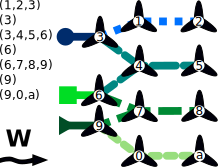
\includegraphics[width=0.7\columnwidth]{wind.pdf}
\caption{Wind farm setup. The incoming wind is denoted by an arrow. Each local group is denoted by a
different color and line type. Groups are listed explicitly on the left. Note the three single-agent
groups on the left to handle per-agent rewards.}
\label{fig:wind_graph}
\end{figure}

In our wind farm experiment, we used a state-of-the-art simulator \cite{vandijk2016} to mimic the energy production of a series of wind turbines when exposed to a global incoming wind vector. In the real world, turbines can often be oriented at certain angles to maximize production. This is a non-trivial control task, as the turbulence caused by a turbine will negatively affect turbines downwind. The direction of this generated turbulence depends on the angle that the turbine has w.r.t. the incoming wind vector.

We setup our simulated wind farm using 11 turbines (see Figure~\ref{fig:wind_graph}). Each turbine has a
choice between three different actions (angles) that it can turn to. The last $4$ turbines downwind (2, 5, 8, and $a$)
are set directly against the wind and are not controlled by agents, as they cannot generate
turbulence that can impact power production. However, the remaining $7$ turbines do influence the
rest of the farm, and so must cooperate to maximize power production.

\begin{figure*}[ht!]
\centering
\subfigure[0101-Chain, All Algorithms]{\label{fig:nodes_all}\includegraphics[width=0.49\columnwidth]{nodes_all.png}}
\subfigure[0101-Ch., MAUCE\&SCQL]{\label{fig:nodes_xs}\includegraphics[width=0.49\columnwidth]{nodes_xs.png}}
\subfigure[Gem Mining]{\label{fig:mines}\includegraphics[width=0.49\columnwidth]{mines.png}}
\subfigure[Wind Farm]{\label{fig:wind}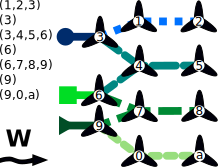
\includegraphics[width=0.49\columnwidth]{wind.png}}
%\subfigure[0101-Chain, All Algorithms]{\label{fig:nodes_all}\includegraphics[width=0.49\columnwidth]{nodes1.pdf}}
%\subfigure[0101-Ch., MAUCE\&SCQL]{\label{fig:nodes_xs}\includegraphics[width=0.49\columnwidth]{nodes2.pdf}}
%\subfigure[Gem Mining]{\label{fig:mines}\includegraphics[width=0.49\columnwidth]{mines3.pdf}}
%\subfigure[Wind Farm]{\label{fig:wind}\includegraphics[width=0.49\columnwidth]{wind4.pdf}}
\caption{Cumulative regret for all experiments as a function of the number of actions executed: a)
0101-Chain averaged over 100 runs, b) Same as \ref{fig:nodes_all}, only SCQL and MAUCE, c) Gem
Mining, averaged over 5 random setups, 100 runs per setup, and d) Wind Farm, 10 runs. }
\label{fig:nodes_results}
\end{figure*}

We vary the wind speed in the simulator at each timestep, following a truncated normal distribution
with mean $8.1$ m/s. The overall reward is normalized to a $[0, 1]$ interval using the maximum
possible overall reward at the highest wind strength and the minimum possible reward per turbine at
the minimum wind strength. While this makes it impossible to compute the true regret, as choosing
the optimal action does not result in a $0$ regret in expectation, it avoids having to calculate the
true expected reward for all actions in this scenario, which is non-trivial.

Differently from the previous experiments, rewards in this settings are obtained per-agent from the
simulator rather than per-group. Thus, we use single-agent local groups to prevent dependencies
between the reward functions of each group. The reward for agents in more than one group is given
solely to their single-agent group, and none to the others (rather than splitting).

\subsection{Results}

We tested the performance of MAUCE on the higly structured 0101-Chain problem with 11 agents for
10,000 joint action executions, and compare its performance against random, SCQL and LLR. The
results (Figure \ref{fig:nodes_results}) indicate that both SCQL and MAUCE can learn effectively,
far outclassing random joint action selection and LLR.

When comparing MAUCE and SCQL (Figure \ref{fig:nodes_xs}), MAUCE achieves considerably less regret than SCQL. This is because MAUCE's exploration strategy is based on the aggregation of local exploration bounds, while SCQL uses an $\varepsilon$-greedy exploration strategy. On the other hand, SCQL does learn the optimal joint action quickly, thanks to optimistic initialization and this aggressive exploration strategy. We note that after a while, we decreased $\varepsilon$ to $0$, i.e., only exploit, making the regret graph a flat line from that point onward. We note that the annealing of $\varepsilon$ needed to be fine-tuned.
We thus conclude that MAUCE is an effective algorithm that can exploit the graphical structure, leading to superior performance for this highly-structured problem.

We then tested MAUCE against the other algorithms on randomly generated Gem Mining instances with 5
villages and 8 mines, to compare performances on a more challenging problem. Figure \ref{fig:mines}
represents the average regret over multiple different scenarios. We observe that, while SCQL and LLR
are all able to achieve sublinear regret curves, MAUCE handles the exploration-exploitation
tradeoffs best, resulting in the lowest regret over time.

Finally, to test the performance of MAUCE on a real-world problem, we run the algorithms on a Wind
Farm instance (Figure \ref{fig:wind}). Due to the high computational costs of running the simulator,
we perform only ten runs. As explained before, the measure shown is not an exact form of regret, as
the optimal action will not result in a $0$ regret in expectation.

The MAUCE algorithm once again performs best, with less cumulative regret than both LLR and SCQL.
The LLR algorithm also doesn't seem to achieve any significant learning with respect to the random
policy. Note that MAUCE keeps learning and fine tuning this policy over the whole duration of the
experiment, which allows it to increasingly achieve lower regret than SCQL. At timestep 10000, the
difference between the two is $43.258$, while at timestep 40000 it is $81.373$.  It is important to
note that SCQL could probably be made to perform better by finely tuning the initialization values
and epsilon updates, but this would take significant human time and repetitive trials. MAUCE can
instead directly manage the exploration-exploitation trade-off by using its local bounds for each
local joint action.

We thus conclude that MAUCE is an effective algorithm for trading off exploration versus exploitation in MAMABs, and has superior performance w.r.t.\ the alternative algorithms.

 %SCQL on the other hand, while it can be less performant due to the difficulty of correctly setting up its exploration methods, can be more resilient when dealing with unknown problems as it is harder to mess up optimistic initialization and an epsilon policy.

%\textcolor{blue}{(Timo: how many times have these experiments been run?)}
